\documentclass{dependencies/acm_proc_article-sp}

\usepackage{url}
\usepackage{color}
\usepackage{verbatim}
\usepackage{listings}
\lstset{
  language=C++,         	% choose the language of the code
  basicstyle=\small,   	% the size of the fonts that are used for the code
  numbers=left,               	% where to put the line-numbers
  numberstyle=\footnotesize,  	% the size of the fonts that are used for the line-numbers
  stepnumber=0,               	% the step between two line-numbers. If it is 1 each line will be numbered
  numbersep=5pt,              	% how far the line-numbers are from the code
  backgroundcolor=\color{white},  % choose the background color. You must add \usepackage{color}
  showspaces=false,           	% show spaces adding particular underscores
  showstringspaces=false,     	% underline spaces within strings
  showtabs=false,             	% show tabs within strings adding particular underscores
  %frame=single,               	% adds a frame around the code
  tabsize=2,          	% sets default tabsize to 2 spaces
  captionpos=t,               	% sets the caption-position to bottom
  breaklines=false,    	% sets automatic line breaking
  breakatwhitespace=false,	% sets if automatic breaks should only happen at whitespace
  escapeinside={\%}{)}      	% if you want to add a comment within your code
}

% Get rid of the permission block
\makeatletter
\let\@copyrightspace\relax
\makeatother

\begin{document}

\title{ Distrivia: A Distributed Trivia Game }
\numberofauthors{3}
\author{
\alignauthor
Brian Gianforcaro \\
   	\affaddr{Rochester Institute of Technology}\\
   	\email{bjg1955@rit.edu}
\alignauthor
Steven Glazer \\
   	\affaddr{Rochester Institute of Technology}\\
   	\email{sfg6126@rit.edu}
\alignauthor
Samuel Milton \\
   	\affaddr{Rochester Institute of Technology}\\
   	\email{srm2997@rit.edu}
}
\maketitle

\begin{abstract}
In this paper we will discuss our decisions and detail our discoveries throughout designing a distributed trivia system, Distrivia.
This paper will outline our motivations behind the project, the architecture, design, implementation, lessons learned, and future work for the distributed trivia system.
The distrivia system was implemented on 3 platforms (web, Android, and iPhone) to provide multiple ways for players to stay connected.
It also utilizes advanced distributed systems algorithms and technology such as Amazon's EC2, Riak, SSL communication, round robin DNS, and NGINX load sharing.
All of these services provide for high availability and secure play.
\end{abstract}

\section{Project Motivation}
Our motivation for this project was to build a system that would allow people to compete across multiple platforms reliably.
High availability was a major concern for us, as it enables people to compete at all times.
This form of trivia is a multi player social game.
It takes advantage of a number of different platforms so that users can feel free to play on any device they prefer.
The web client ensures that almost any device will be able to connect and play.
Designing it on mobile platforms allows us to take advantage of the specific platform and lets people easily play on the go.

\section{Architecture}
\subsection{Servers}
For our servers, we used Amazon EC2 micro instances,  running x86-64 custom Amazon Linux.
They each have 8GB of network attached storage and 613MB of memory.

Each server is installed with our custom web app that services our requests.
They are  also equipped with an instance of Riak \cite{riak} which is our database back end of choice for persisting game and player. Our Python web app utilizes the Flask \cite{flask} web framework and we serve this application and all application content with the Tornado \cite{tornado} web server, both of which are open source.

For load sharing, we used the NGINX \cite{nginx} web server in a reverse proxy configuration. This service can be used on any machine with an active Internet connection and the ability to receive connections on port 80 for HTTP and port 443 SSL. 


\section{Design}
\begin{figure}[h!]
  \centering
	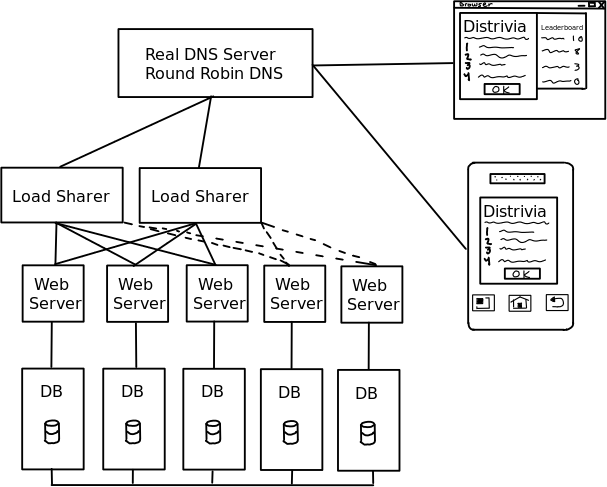
\includegraphics[scale=0.4]{diagram.png}
   \caption{High level overview of the system}
 \end{figure}
\subsection{Servers}
As previously mentioned, each server contains the server application that responds to clients as well as the Riak databases.
Riak handles auto-synchronization of the databases between any connected servers.
This allows for data to be transparently transferred and replicated across all server-nodes in the ring.
Servers can easily be added and removed from the ring by updating Riak.
When Riak is updated, the current nodes will either start updating any new nodes or stop communicating with any nodes that are no longer in the ring, according to the new update.
These servers, therefore, all contain the same information.
If any servers go down, the distributed system would still run fine.
This configuration allows for all servers go down except one and the system would still be reliably handling requests.

\subsection{Server Applications}
The server application handles requests from the user via the load sharers.
Interpretation of the client messages and replies are handled by the applications. There is one application per server processing requests and responding via https messages with JSON objects. Requests are formed using a REST like API, where the URL is the method we want to invoke. The parameters to the method's are passed in through a HTTP POST. The server processes the request reading or writing to the data store and returns the appropriate data in JSON format. This system is basically an abstracted RPC system, composed of two different web technologies. Every request to the API is checked for proper authentication. Authentication is handled by generating a unique token for each user login, which they need to pass along with each request. This method avoids the possibility of potential security vulnerabilities from passing the users password around more than needed. 
The server application supports the following features:
\begin{itemize}	
\item Client registration
\item Login
\item Query games status
\item Joining public games
\item Joining private games
\item Creating private games
\item Question retrieval
\item Question answering
\item Global leader board
\end{itemize}

The database back end was designed for high availability and durability of the game data. For every write to the data store, all other online nodes must agree with the write for it to be committed. In this way we can make sure that their is total consistency in the database at all times, reducing the risk of database corruption. 

\subsection{Load Sharers}
The load sharers act as an agent between the clients and the servers to ensure reliable, fast communication. Messages are relayed through the load sharers from the client. Once received, the load sharer will pass the message onto any active server or, if there are none active, it will deliver the message to a hot spare server. This is an important part of the distributed system in keeping network traffic down on the active servers so they may serve requests faster and for making sure the server attempting to service the client's request is active and able to process the message.They attempt to connect to a server twice in a one second period before deeming it dead and removing it from its list of servers to direct clients towards. This is important to make sure that any servers that go down do not receive further communication attempts.


\subsection{Clients}
Distrivia is designed for three distinct platforms (web, Android, and iPhone).
The clients were designed to run on each platform without specific hardware or relying on external applications.
The clients can be run, once installed, from desktop computers, laptops, Androids, and iPhones out of the box.
The web client can be run from any browser that supports CSS and javascript, which is true of all modern graphical web browsers. This gives users of other mobile phones, such as Blackberrys or Palm Pres, the ability to play even though there is not a native app for them. The Android client will run on any Android platform running OS 2.1 or higher and does not use any unique services that require specific hardware. Likewise, the iPhone client will run on any iPhone/iPod touch platform running any iOS without the need for specific hardware. The Android and iPhone clients just require an active data connection either by cell signal or wireless Internet.

All of our clients were designed similarly.
We tried to keep the layout as simple as possible, for the user to be able to easily navigate the game.
The mobile clients are the quite similar due to their similar and limited screen real estate.
This was important in allowing players to play on multiple platforms while using a layout they were used to.
As mobile gaming continues to grow, our approach was to promote the play of Distrivia on the go.
Each round can be quickly played within the course of a few minutes, which makes it ideal for playing on mobile devices.
Distrivia allows users to connect with players on any other device which gives friends the opportunity to play together without forcing them to conform to one platform.

The clients are broken down into 4 distinct views/activities: login, join, compete, and view leader board. 
Login provides the player with a way to access the game using a username/password combination.  From the same screen, a user can create a new account, which will automatically log them in after creation.
Once the player has been verified, the client will progress to the join screen. 
The join screen allows players to pick from joining public games, joining/creating private games, or viewing the global leader board. 
Once a user requests to join a game (private or public) the client will request status updates from the server about the progress of the game.
These status queries occur every 5 seconds, allowing time for the server to respond without becoming overloaded. 
Once the game has enough players to start, the client is alerted through these status queries and the clients progress to the competition screen.
During competition, the players is presented with the question and a set of possible answers.
The player can then read, select an answer, and submit the answer using the “Submit” button.
The screen will then be updated with the new scores and the next question/answers until the end of the round.
Once the player reaches the end of a round, the player is shown the local leaderboard for the round and transported back to the join screen for them to join another game.

A large portion of designing the clients was devoted to allowing easy navigation for players without overloading the servers with requests.
There are a couple points during game play where the client is requesting “constant” information to interactively keep updated.
During these occasions, the clients pause for 5 seconds before querying the system again as to not confuse the clients.

\subsection{Messages}
Distrivia uses the https protocol for communication.
This provides a secure and usable messaging system that both the client and server APIs use.
The actual messages are sent and received in two ways.
Initially a user session key is generated using the UUID\cite{uuid} algorithm and returned to the user on successful authentication.
This session key is then passed back to the server with every sent message.
Messages are sent to the server using POST request methods supported by the HTTP protocol.
Responses from the server are in the form of JSON \cite{json} objects.
JSON is a small, easily-parseable format, representing objects in a human readable format as they would be represented in JavaScript.
With the web client the JSON object returned from the server is instantly usable, however for other applications, parsing the JSON object into native objects is necessary.
The Android Software Development Kit provides libraries to do this, located in the org.json \cite{orgjson} package name space.
This was also accomplished for iOS by parsing JSON objects to native Objective-C objects using the JSONKit \cite{objcjson} package developed by John Engelhart.

\section{Implementation}
\subsection{Network}
For the implementation of Distriva, we deployed six servers on Amazon's Elastic Compute Cloud \cite{aec} to run the server application and host the databases.
One server is being used as a web-monitor host running Monit\cite{monit}.
We were able to log in to the web-monitor to see the status of all our servers, databases, and load sharers. 
This assisted us in managing whether or not the services were running and allowed us to track down any problems when they arose.
Three of the servers were set up as active, front facing servers for clients to query.
The two other servers were set up as hot spares, in case of a failure. 
The hot spares were set up to be part of the database cluster so they have a full copy of the database on hand, however they did not accept any reads or writes directly unless the load sharers found no active servers are responding. 
In the event of such a failure the load distributor would automatically fail over and start relaying the client messages to the hot spares. 
Since both hot spares are members of the database cluster they already would have the most up-to-date game information information.

For this project, we set up two load sharers which are running on personal desktop computers with reliable Internet connections.
The duplicate sharers allow for a load sharer to go down and we would still be able to serve requests to the servers.
These are set up with round robin DNS entries, courtesy of ZoneEdit.com \cite{zoneedit}, a free DNS management service.
These load sharers are selected by the clients where distrivia.lame.ws will select either load distributer that is up at random.
If a load distributer should go down or become unreachable the DNS service will no longer serve that hosts DNS record until it is again reachable.
This provides us with stability for accessing the servers.

\subsection{Clients}
We implemented the Distrivia applications on multiple platforms.
For the web client, we used Chrome, Firefox, Safari, and Internet Explorer.
Using these different web browsers, we were successfully able to compete with users on other browsers and devices.
For the mobile platforms we implemented the native Distrivia apps for Android and iPhone.
Creating native apps for Android and iPhone gives the users the best performance on those devices along with the native look and feel of the device for optimal design.
Playability on all clients was similar and easy to navigate. Shown below are screenshots from the various implementations of the Distrivia project.
\begin{figure}[h!]
   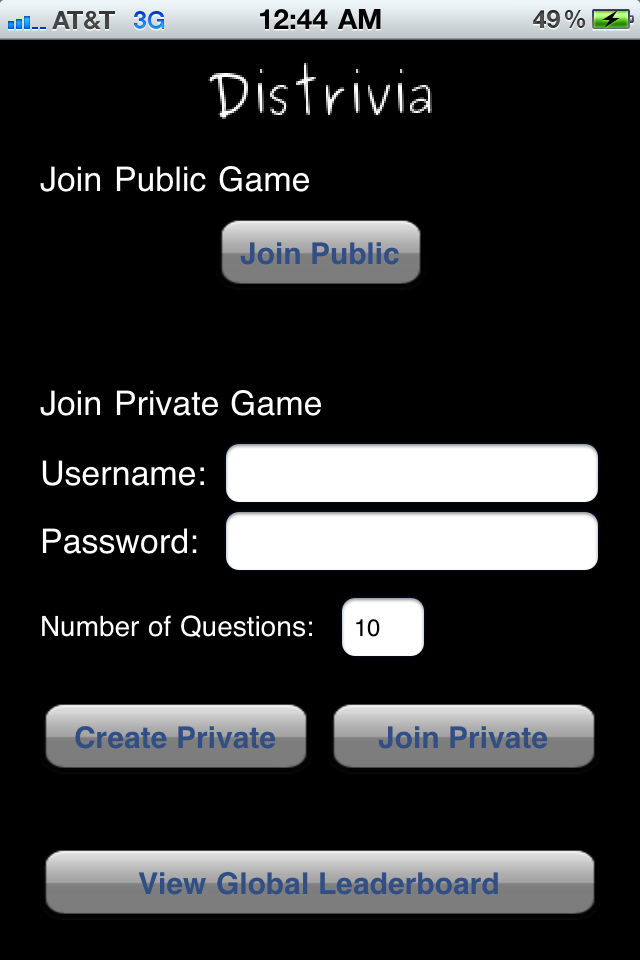
\includegraphics[scale=0.12]{iPhone_join.png}
   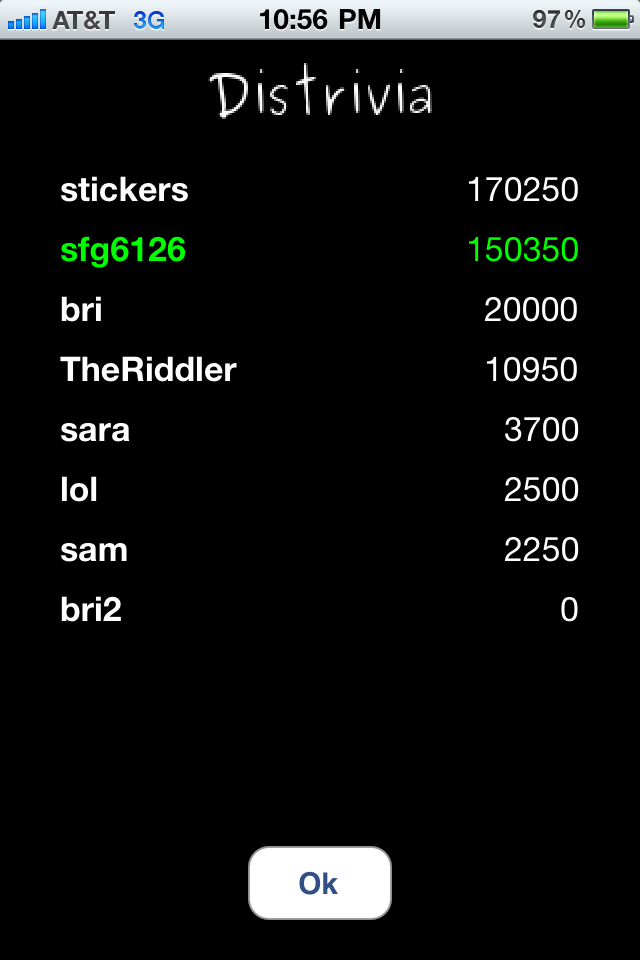
\includegraphics[scale=0.12]{iPhone_leaderboard2.png}
   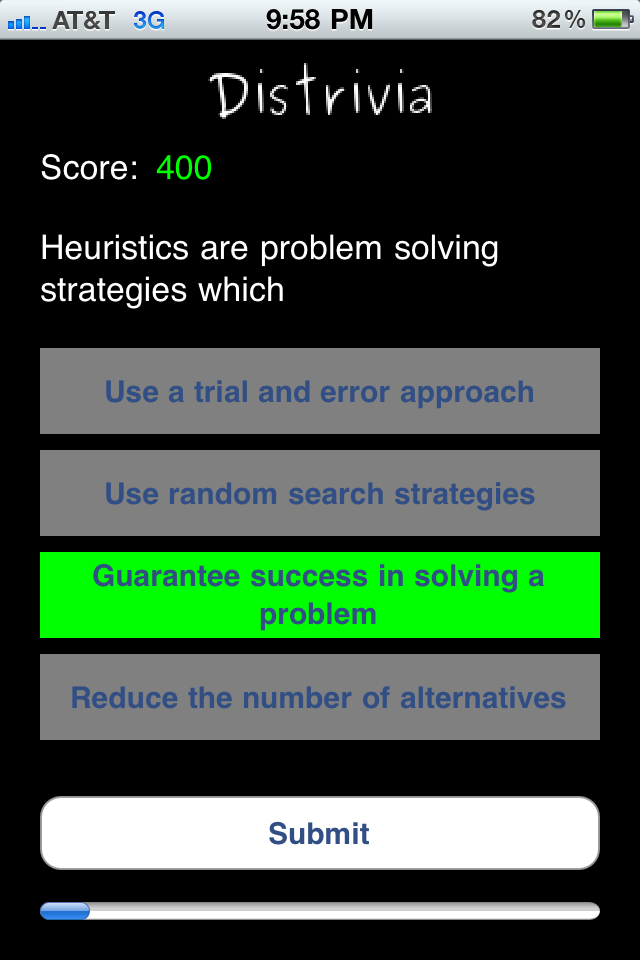
\includegraphics[scale=0.12]{iPhone_round.png}
   \caption{iPhone Client User Interface}
\end{figure}

\begin{figure}[h!]
   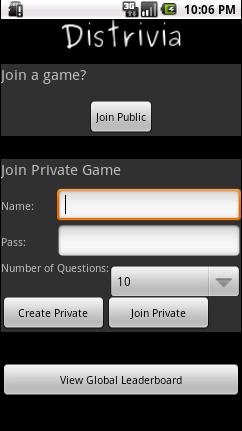
\includegraphics[scale=0.32]{android/join.png}
   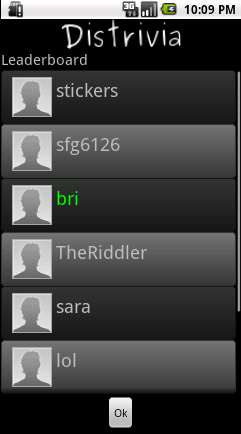
\includegraphics[scale=0.32]{android/lb.png}
   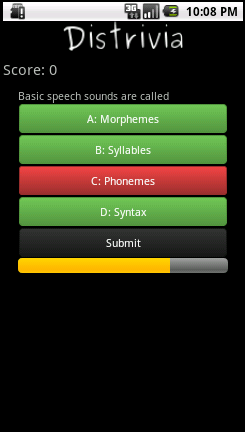
\includegraphics[scale=0.32]{android/answer2.png}
   \caption{Android Client User Interface}
\end{figure}

\begin{figure}[h!]
   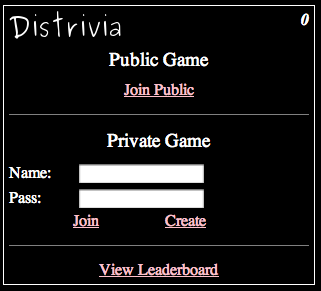
\includegraphics[scale=0.21]{web_join.png}
   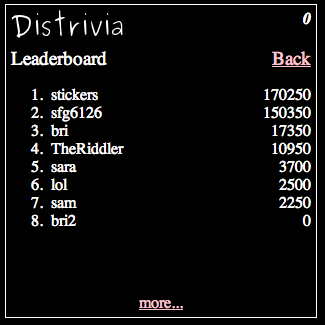
\includegraphics[scale=0.21]{web_leader.png}
   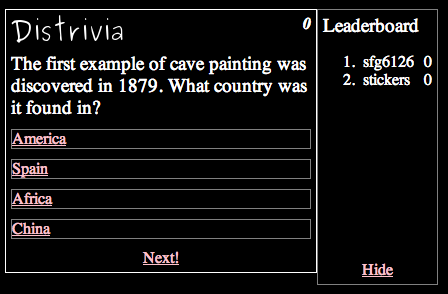
\includegraphics[scale=0.21]{web_round.png}
   \caption{Web Client User Interface}
\end{figure}


\section{Lessons Learned}
One of the first lessons we learned during this project was the concept that you can't have high performance, durability, and availability.  For our system which does not have to do a significant amount of computation for each user request, we decided to sacrifice performance in favor of durability and availability.  The computations are very quick and simple, and we think users would rather have a potentially slow service than an unavailable service.  

While it was a concept we were already familiar with, the importance of consistency was heavily ingrained into us.  During development, we frequently ran into trouble where our clients would start off communicating with one server and then switch later.  Our client would then often start getting errors because the new server didn't recognize the authentication key.  As a result we had to go back and really make sure our servers stayed consistent so that when clients end up talking to a different server the communications without interruption.  It also made us realize just how hard it can be to keep multiple computers synchronized at all times.

\section{Future Work}
For future work on this system, we've thought of adding a few new features that would improve gameplay and diversity of the experience for the players.
We don't have have any revolutionary upgrades we'd like to perform on the server-side.
Overall, we are satisfied with the performance of the server including the reliability, response speed, and availability. The features we have contemplated adding in future work include: categories, user added content, support for more platforms, and private competition via bluetooth or local wifi.

Distrivia randomizes the questions in all categories and sets up each game to have these randomized groupings.
It would be nice, in the future, to support the feature of players being able to choose from a list of categories to compete in.
This would allow players to compete in areas that they feel most comfortable in or to try out new categories to really test their trivia prowess.

Another feature to look into would be allowing users to submit their own questions/answers to the server for other players to play.
This would help build the database and get a broader range of questions.
There would need to be some sort of interactive rating system so that players can rate user-added question so that if the question were rated low enough, it would no longer be included in future games.
For a different approach, the player may only be able to use custom questions in private rounds with their friends so that the questions wouldn't need to be monitored or rated.

Distrivia currently runs natively on two mobile platforms.
It would be preferred if this could be expanded to more platforms to allow for a broader range of users to participate.
Using the current framework, it would not be much more effort to add native applications for blackberrys, palm devices, Android tablets, and iPads.
Android tablets and iPads would be interesting devices to add support for since they allow utilization of larger screen space.
This would allow the user to be able to see full local leader boards while competing in each round, as well as other upgraded viewing options from the smaller mobile devices.

Lastly, support for bluetooth connected play and local wifi play would add even greater support for private gameplay. 
It would also make it so that devices would not need connections to the Internet to participate.
This means that non-data devices such as iPods could play without access to wifi.
It would also allow users in data dead-zones to participate and play with their friends.

\newpage
%
% The following two commands are all you need in the
% initial runs of your .tex file to
% produce the bibliography for the citations in your paper.
\bibliographystyle{abbrv}
\bibliography{bibliography}  % sigproc.bib is the name of the Bibliography in this case
% You must have a proper ".bib" file
%  and remember to run:
% latex bibtex latex
% to resolve all references
%
% ACM needs 'a single self-contained file'!
%
%APPENDICES are optional
\balancecolumns
% That's all folks!
\end{document}

